\documentclass[a4paper,12pt]{article} 
\usepackage[utf8]{inputenc} % Acentos válidos sin problemas
\usepackage[spanish]{babel} % Idioma
%\usepackage[style=biber]{biblatex}
%\addbibresource{bibliografia.bib}
%\usepackage[
%  backend=biber
%]{biblatex}
\usepackage[backend=biber, style=ieee]{biblatex}
\addbibresource{bibliografia.bib}
\usepackage{csquotes}
%\usepackage{background}
%\setlegtth{\parindent}{2px}
%\phantom{abc}
\usepackage{csvsimple}
\usepackage{filecontents}
%\usepackage{json}
%\usepackage{fancyvrb}


%-----------------------------------INICIO DE PACKETES------------------/
%----------------------------------------------------------------------/|
\usepackage{amsmath}   % Matemáticas: Comandos extras(cajas ecuaciones) |
\usepackage{amssymb}   % Matemáticas: Símbolos matemáticos              |
\usepackage{datetime}  % Agregar fechas                                 |
\usepackage{graphicx}  % Insertar Imágenes                              |
\usepackage{biblatex} % Bibliografía                                   |
\usepackage{multicol}  % Creación de tablas                             |
\usepackage{longtable} % Tablas más largas                              |
\usepackage{xcolor}    % Permite cambiar colores del texto              |
\usepackage{tcolorbox} % Cajas de color                                 |
\usepackage{setspace}  % Usar espacios                                  |
\usepackage{fancyhdr}  % Para agregar encabezado y pie de página        |
\usepackage{lastpage}  %                                                 |
\usepackage{float}     % Flotantes                                      |
\usepackage{soul}      % "Efectos" en palabras                          |
\usepackage{hyperref}  % Para usar hipervínculos                        |
\usepackage{caption}   % Utilizar las referencias                       |
\usepackage{subcaption} % Poder usar subfiguras                         |
\usepackage{multirow}  % Nos permite modificar tablas                   |
\usepackage{array}     % Permite utilizar los valores para multicolumn  |
\usepackage{booktabs}  % Permite modificar tablas                       |
\usepackage{diagbox}   % Diagonales para las tablas                     |
\usepackage{colortbl}  % Color para tablas                              |
\usepackage{listings}  % Escribir código                                |
\usepackage{mathtools} % SIMBOLO :=                                     |
\usepackage{enumitem}  % Modificar items de Listas                      |
\usepackage{tikz}      %                                                |
\usepackage{lipsum}    % for auto generating text                       |
\usepackage{afterpage} % for "\afterpage"s                              |
\usepackage{pagecolor} % With option pagecolor={somecolor or none}|     |
\usepackage{xpatch}    % Color de lineas C & F
%\usepackage{glossaries} %                                             
\usepackage{lastpage}       





%----------------------------------------------------------------------\|
%-----------------------------------FIN--- DE PACKETES------------------\
%\usepackage{listings}
%\lstset{
%  language=Scheme
%}

%--------------------------------/
%-------------------------------/
\usepackage[                 %   |
  headheight=15pt,  %            |
  letterpaper,  % Tipo de pag.   |
  left =1.5cm,  %  < 1 >         |
  right =1.5cm, %  < 1 >         | MARGENES DE LA PAGINA
  top =2cm,     %  < 1.5 >       |
  bottom =1.5cm %  < 1.5 >       |
]{geometry}     %                |
%-------------------------------\
%--------------------------------\

%----------------------------------------------------------------------/
%-------------------Encabezado y Pie de Pagina-----------------------/ |
%--------------------------------------------------------------------\ |
%\fancyhf{}           %                                                |

     %                                                |
%\pagestyle{fancy}

\fancypagestyle{firstpage}{  
  \fancyfoot[L]{\textsc{\textcolor{white}{\small {Fundamentos de Bases de Datos}}}}
  \fancyfoot[C]{}
  \fancyfoot[R]{\textcolor{white}{\thepage\ de \pageref*{LastPage}}} 
  \renewcommand{\footrulewidth}{1.5pt} %     | 
\xpretocmd\footrule{\color{white}}{}{\PatchFailed}
}

\fancypagestyle{fancy}{  

\fancyhead[L]{{\textcolor{white}{2024-1}}} %                         
\fancyhead[R]{\textcolor{white}{}}     % |
\fancyfoot[L]{\textsc{\textcolor{white}{\small {Fundamentos de Bases de Datos}}}}
  \fancyfoot[C]{}
  \fancyfoot[R]{\textcolor{white}{\thepage\ de \pageref*{LastPage}}} 
\renewcommand{\headrulewidth}{1pt} %
\xpretocmd\headrule{\color{white}}{}{\PatchFailed}
\renewcommand{\footrulewidth}{1.5pt} %     | 
\xpretocmd\footrule{\color{white}}{}{\PatchFailed}

}


%--------------------------------------------------------------------\ |
%-------------------Encabezado y Pie de Pagina-----------------------/ |
%------------------------------------------------------------FIN----/

%--------------------------------------------------------------------\ |
%------------------- LISTA DE COLORES -------------------------------/ |
\definecolor{ProcessBlue}{RGB}{0,176,240}
\definecolor{NavyBlue}{RGB}{0,110,184}
\definecolor{Cyan}{RGB}{0,174,239}
\definecolor{MidnightBlue}{RGB}{0,103,49}
\definecolor{ForestGreen}{RGB}{0,155,85}
\definecolor{Goldenrod}{RGB}{255,223,66}
\definecolor{YellowGreen}{RGB}{152,204,112}
\definecolor{Sepia}{RGB}{103,24,0}
\definecolor{Peach}{RGB}{247,150,90}
\definecolor{CarnationPink}{RGB}{242,130,180}
\definecolor{Fuchsia}{RGB}{140,54,140}
\definecolor{WildStrawberry}{RGB}{238,41,103}

\definecolor{Grass}{RGB}{41,238,53}
\definecolor{Meadow}{RGB}{6,243,67}
\definecolor{jellyfish}{RGB}{109,14,130}
\definecolor{rubber}{RGB}{229,27,232}
\definecolor{bullet}{RGB}{225,31,90}
\definecolor{midnight}{RGB}{31,90,225}
\definecolor{sun}{RGB}{241,152,7}
\definecolor{water}{RGB}{16,229,183}
%------------------- LISTA DE COLORES -------------------------------/ |
%----------------------------------------------------------------------/

\usepackage{tikz,times}
\usepackage{verbatim}
\usetikzlibrary{mindmap,trees,backgrounds}

\definecolor{color_mate}{RGB}{255,255,128}
\definecolor{color_plas}{RGB}{255,128,255}
\definecolor{color_text}{RGB}{128,255,255}
\definecolor{color_petr}{RGB}{255,192,192}
\definecolor{color_made}{RGB}{192,255,192}
\definecolor{color_meta}{RGB}{192,192,255}

\lstdefinelanguage{json}{
    basicstyle=\color{white}\normalfont\ttfamily,
    numbers=left,
    numberstyle=\scriptsize,
    stepnumber=1,
    numbersep=8pt,
    showstringspaces=false,
    breaklines=true,
    frame=lines,
    backgroundcolor=\color{black},
    literate=
     *{0}{{{\color{blue!50!white}0}}}{1}
      {1}{{{\color{blue!50!white}1}}}{1}
      {2}{{{\color{blue!50!white}2}}}{1}
      {3}{{{\color{blue!50!white}3}}}{1}
      {4}{{{\color{blue!50!white}4}}}{1}
      {5}{{{\color{blue!50!white}5}}}{1}
      {6}{{{\color{blue!50!white}6}}}{1}
      {7}{{{\color{blue!50!white}7}}}{1}
      {8}{{{\color{blue!50!white}8}}}{1}
      {9}{{{\color{blue!50!white}9}}}{1}
      {:}{{{\color{orange!70!black}{:}}}}{1}
      {,}{{{\color{orange!70!black}{,}}}}{1}
      {\{}{{{\color{red!60!black}{\{}}}}{1}
      {\}}{{{\color{red!60!black}{\}}}}}{1}
      {[}{{{\color{red!70!white}{[}}}}{1}
      {]}{{{\color{red!70!white}{]}}}}{1},
}

\begin{document}%----------------------INICIO DOCUMENTO------------|
%------------------------------------------------------------------|
\pagecolor{black}
\color{white}

\thispagestyle{firstpage} % Aplicar estilo de primera página
\noindent
%%%%%%%%%%%%%%%%%%%%%%%%%%%%%%%%%%%%%%%%%%%%%%%%%%%%%%%%%%%%%%%%%%%%%%%%%%%%%%
\large\textbf{Facultad de Ciencias} \\
Fundamentos de Bases de Datos \hfill semestre: 2024-1 \\
\textsc{SILVA HUERTA MARCO}   \hfill No.Cuenta: 316205326    \\
11 de Septiembre de 2023      \hfill \textbf{Practica \#02}    \\
\noindent\rule{7.3in}{2.8pt}
%%%%%%%%%%%%%%%%%%%%%%%%%%%%%%%%%%%%%%%%%%%%%%%%%%%%%%%%%%%%%%%%%%%%%%%%%%%%%%

\begin{center}
\Large{Modelos de datos}
\end{center}

\subsection*{Objetivo}
Que el alumno genere modelos orientados a objetos, relacional y semiestructurado y
refuerce el conocimiento visto en clase.

\subsection*{Instrucciones}

Los modelos de datos nos ayudan a describir la estructura de una base de datos, brindando
los medios necesarios para lograr la abstracción de los datos. Tres principales modelos que
abordaremos son:\\

El modelo orientado a objetos almacena y manipula información que puede ser presentada 
como objetos; las llamadas bases de datos orientadas a objetos \textbf{(BDOO)} pueden manejar
herencia, polimorfismo y encapsulamiento. (No está incluido en esta práctica).\\

El modelo semiestructurado surge ante la necesidad de que cada elemento almacenado
cuente con un conjunto de atributos propio, sin necesidad de que este conjunto sea
obligatorio como sucede en el modelo relacional. Este tipo de bases de datos se crea con el
lenguaje de marcado extensible XML.

\newpage
\thispagestyle{fancy} % Aplicar estilo de primera página


\subsection*{Ejercicio 1}

Modelo semiestructurado

Deberás leer el archivo csv de la práctica 1 y pasarlo a alguna estructura del modelo
semiestructurado (json, xml, html etcétera), recomiendo json por ser el más usado.


\subsubsection*{Archivo CSV}

\begin{filecontents*}{productos.csv}
    ID,Nombre,Categoria,Precio,Cantidad en Existencia
    AMOANA,Amoxicilina,Antibióticos,150.0,24
    IBUAOS,Ibuprofeno,Analgésicos,50.0,50
    PARAOS,Paracetamol,Analgésicos,30.0,100
    OMEOOS,Omeprazol,Otros,20.0,30
    ASPAOS,Aspirina,Analgésicos,40.0,60
    VITAOS,Vitaminas,Alimentos,15.0,200
    AGUBAS,Agua Mineral,Bebidas,5.0,120
    CREHTE,Crema Hidratante,Desinflamantes,25.0,40
    JABOOS,Jabón de Manos,Otros,8.0,75
    SUEBAS,Suerox,Bebidas,20.0,20
    SUEBAS,Suerox,Bebidas,15.5,10
\end{filecontents*}

\csvautotabular{productos.csv}

\subsubsection*{Archivo CSV}

%\jsonfile{productos.json}

\begin{lstlisting}[language=json, caption=productos.json]
    {
        [
            {
              "ID": "AMOANA",
              "Nombre": "Amoxicilina",
              "Categoria": "Antibioticos",
              "Precio": 150.0,
              "Cantidad en Existencia": 24
            },
            {
              "ID": "IBUAOS",
              "Nombre": "Ibuprofeno",
              "Categoria": "Antibioticos",
              "Precio": 50.0,
              "Cantidad en Existencia": 50
            },
            {
              "ID": "OMEOOS",
              "Nombre": "Omeprazol",
              "Categoria": "Otros",
              "Precio": 20.0,
              "Cantidad en Existencia": 30
            },
            {
              "ID": "ASPAOS",
              "Nombre": "Aspirina",
              "Categoria": "Analgesicos",
              "Precio": 40.0,
              "Cantidad en Existencia": 60
            },
            {
              "ID": "VITAOS",
              "Nombre": "Vitaminas",
              "Categoria": "Alimentos",
              "Precio": 15.0,
              "Cantidad en Existencia": 200
            },
            {
              "ID": "AGUBAS",
              "Nombre": "Agua Mineral",
              "Categoria": "Bebidas",
              "Precio": 5.0,
              "Cantidad en Existencia": 120
            },
            {
              "ID": "CREHTE",
              "Nombre": "Crema Hidratante",
              "Categoria": "Desinflamantes",
              "Precio": 25.0,
              "Cantidad en Existencia": 40
            },
            {
              "ID": "SUEBAS",
              "Nombre": "Suerox",
              "Categoria": "Bebidas",
              "Precio": 15.5,
              "Cantidad en Existencia": 10
            },
            {
              "ID": "LLAOOS",
              "Nombre": "Llavero",
              "Categoria": "Otros",
              "Precio": 15.5,
              "Cantidad en Existencia": 90
            },
            {
              "ID": "PALAOS",
              "Nombre": "Paletas",
              "Categoria": "Alimentos",
              "Precio": 12.0,
              "Cantidad en Existencia": 30
            }
          ]          
    }
\end{lstlisting}


\subsection*{Ejercicio 2}

Modelo relacional

Basándote en las figuras 1.2 y 2.1 diseña un esquema de base de datos y coloca algunos
registros de ejemplo sobre un universo de discurso de tu elección.

\begin{center}
    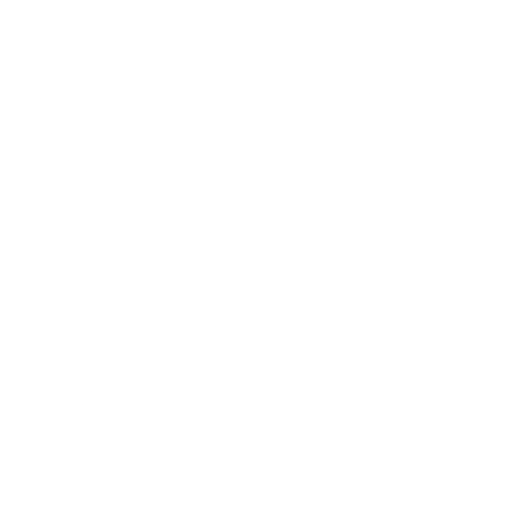
\includegraphics[scale = .6]{ejercico02.png}
\end{center}

\subsection*{Ejercicio 3}

Completa el modelo con los siguientes aspectos:

\begin{enumerate}
    \item ¿Qué tipo de información adicional y restricciones podrías representar en este
    esquema? Inventa al menos 5 restricciones y agrega al menos 5 campos distribuidos
    en distintas tablas, también si lo consideras necesario, puedes agregar una tabla
    adicional.

    \item Menciona al menos 3 usuarios de tu base de datos, define los privilegios que cada
    uno tendría en la BD y describe el tipo de información que cada uno de ellos
    utilizaría.
\end{enumerate}


\section*{Cuestionario}

\begin{enumerate}
    \item ¿Cuáles son las 4 principales características de los modelos orientados a objetos?
    \item ¿Cuáles son las 4 principales propiedades de una relación?
    \item ¿Cuál es la principal diferencia entre el modelo entidad relación y el modelo
    semiestructurado?
    \item Nombra 3 ejemplos en el cual se utilice el modelo orientado a objetos.
    \item Nombra 3 ejemplos en el cual se utilice el modelo entidad relación.
    \item Nombra 3 ejemplos en el cual se utilice el modelo semiestructurado.    
\end{enumerate}


\section*{Tablas}

\begin{table}[h]
    \centering
    \caption{\textcolor{white}{Tabla Estudiante}}
    \label{tabla_estudiante}
    \textcolor{white}{
    \begin{tabular}{|c|c|c|c|} 
    \hline
        Nombre & Numero\_Estudiante & Clase & Departamento \\ \hline
        Juan & 4 & 1 & CS \\ \hline
        Luis & 17 & 2 & CS \\ 
    \hline
    \end{tabular}
    }
\end{table}
\begin{table}[h]
    \centering
    \caption{\textcolor{white}{Tabla Curso}}
    \label{tabla_curso}
    \textcolor{white}{
    \begin{tabular}{|c|c|c|c|}
    \hline
    Nombre\_Curso & Numero\_Curso & Horas & Departamento \\
    \hline
        Introducción a Computación & CS1310 & 4 & CS \\
        Estructura de datos & CS3320 & 4 & CS \\
        Matemáticas Discretas & MATH2410 & 3 & MATH \\
        Bases de datos & CS3380 & 3 & CS \\
    \hline
    \end{tabular}
    }
\end{table}
\begin{table}[h]
    \centering
    \caption{\textcolor{white}{Tabla Sección}}
    \label{tabla_seccion}
    \textcolor{white}{
    \begin{tabular}{|c|c|c|c|}
    \hline
        Numero\_Curso & Semestre & Año & Instructor \\ \hline
        MATH2410 & Otoño & 07 & Smith \\
        CS1310 & Primavera & 08 & Lucas \\
    \hline
    \end{tabular}
    }
\end{table}
\begin{table}[h]
    \centering
    \caption{\textcolor{white}{Tabla Calificaciones}}
    \label{tabla_calificaciones}
    \textcolor{white}{
    \begin{tabular}{|c|c|c|}
    \hline
        Número\_Estudiante & ID\_Seccion & Calificacion \\ \hline
                2      &     1       & A \\
                1      &     2       & B \\
    \hline
    \end{tabular}
    }
\end{table}
\begin{table}[h]
    \centering
    \caption{\textcolor{white}{Tabla Prerrequisitos}}
    \label{tabla_prerrequisitos}
    \textcolor{white}{
    \begin{tabular}{|c|c|}
    \hline
        Numero\_Curso & Numero\_Prerrequisito \\ \hline
        CS1310        & CS3320 \\
    \hline
    \end{tabular}
    }
\end{table}
    


    
%\newpage
%\thispagestyle{fancy} % Aplicar estilo de primera página

%\printbibliography


%\newpage
%\thispagestyle{fancy} % Aplicar estilo de primera página
%\NoBgThispage % Quita el fondo de la pagina

%-----------------------------------------------------------------|
\end{document}%----------------------FIN DEL DOCUMENTO------------| 